%%%%%%%%%%%%%%%%%%%%%%%%%%%%%%%%%%%%%%%%%
% Thin Sectioned Essay
% LaTeX Template
% Version 1.0 (3/8/13)
%
% This template has downloaded from:
% http://www.LaTeXTemplates.com
%
% Original Author:
% Nicolas Diaz (nsdiaz@uc.cl) with extensive modifications by:
% Vel (vel@latextemplates.co1m) 
%
% License:
% CC BY-NC-SA 3.0 (http://creativecommons.org/licenses/by-nc-sa/3.0/)
%
%%%%%%%%%%%%%%%%%%%%%%%%%%%%%%%%%%%%%%%%%

%----------------------------------------------------------------------------------------
%	PACKAGES AND OTHER DOCUMENT CONFIGURATIONS
%----------------------------------------------------------------------------------------

\documentclass[a4paper, 11pt]{article} % Font size (can be 10pt, 11pt or 12pt) and paper size (remove a4paper for US letter paper)

\usepackage[protrusion=true,expansion=true]{microtype} % Better typography
\usepackage{graphicx} % Required for including pictures
\usepackage{float}
\usepackage{wrapfig} % Allows in-line images
\usepackage{amsmath}
\usepackage{algorithm}
\usepackage[noend]{algpseudocode}
\usepackage{pifont}
\usepackage{lipsum}
\usepackage{url}
\usepackage[nottoc,numbib]{tocbibind}

\makeatletter
\def\BState{\State\hskip-\ALG@thistlm}
\makeatother
\usepackage{subcaption}
\captionsetup{compatibility=false}
\usepackage{adjustbox}

\usepackage{mathpazo} % Use the Palatino font
\usepackage[T1]{fontenc} % Required for accented characters
\linespread{1.05} % Change line spacing here, Palatino benefits from a slight increase by default

\usepackage[utf8]{inputenc}
\usepackage[T1]{fontenc}
\usepackage{lmodern} % load a font with all the characters

\providecommand{\keywords}[1]{\textbf{\textit{Keywords:}} #1}

\makeatletter
\renewcommand\@biblabel[1]{\textbf{#1.}} % Change the square brackets for each bibliography item from '[1]' to '1.'
\renewcommand{\@listI}{\itemsep=0pt} % Reduce the space between items in the itemize environments and the bibliography

\renewcommand{\maketitle}{ % Customize the title - do not edit title and author name here, see the TITLE block below
% \begin{flushright} % Right align
\begin{center} 
{\LARGE\@title} % Increase the font size of the title

\vspace{50pt} % Some vertical space between the title and author name

{\large\@author} % Author name
\\\@date % Date

\vspace{40pt} % Some vertical space between the author block and abstract
% \end{flushright}
\end{center}
}



%----------------------------------------------------------------------------------------
%	TITLE
%----------------------------------------------------------------------------------------

\title{\textbf{Real-time Fluid Simulation using Position-Based Dynamics}}

\begin{figure}[H]
    \centering
    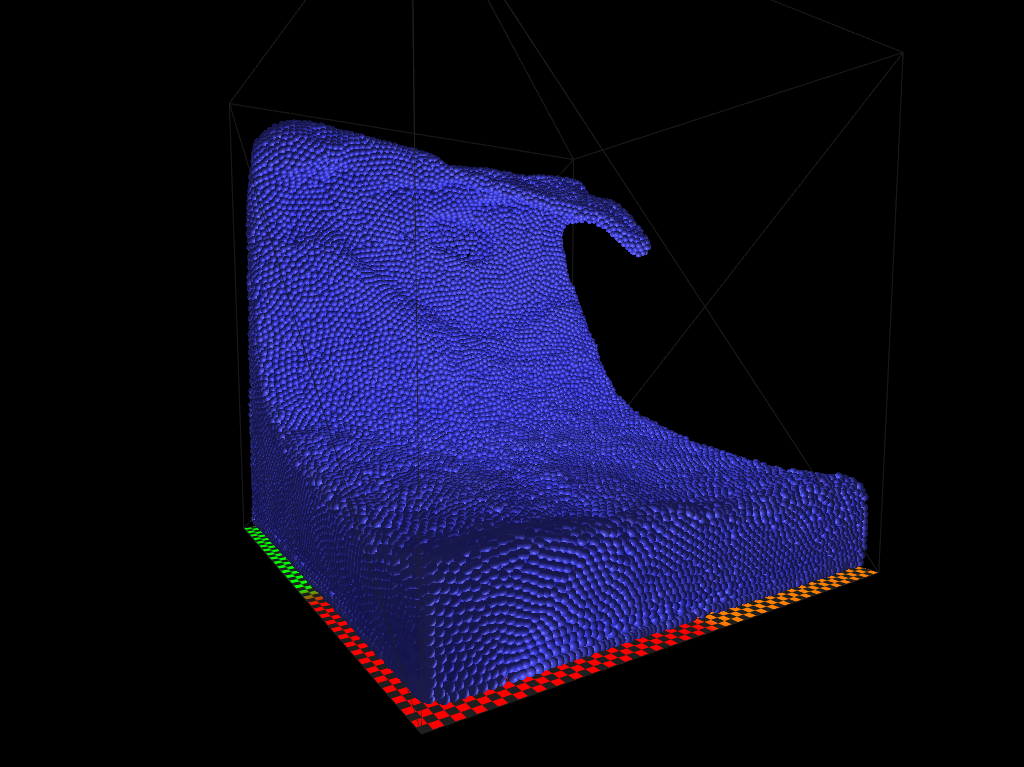
\includegraphics[width=1.0\textwidth]{img/55302_edited.png}
    \label{fig:front}
\end{figure}

% Author
\author{\vspace{-1.2cm}{Niklas Andersson, nikan278},
\\{Gabriel Baravdish, gabba873},
\\{Joakim Deborg, joade361}}


\date{\today} % Date

%----------------------------------------------------------------------------------------

\begin{document}

\maketitle % Print the title section

%----------------------------------------------------------------------------------------
%	ABSTRACT AND KEYWORDS
%----------------------------------------------------------------------------------------

%\renewcommand{\abstractname}{Summary} % Uncomment to change the name of the abstract to something else

\vspace{-1.2cm}

\begin{abstract}
Being able to simulate fluids in real time is important in many applications
including games and interactive visualizations. In this report we describe a
modern approach to modeling fluid behavior at interactive frame rates even on
mediocre hardware. This method is called Position-Based Dynamics and works by
enforcing certain constraints on a set of particles. We also present a method
for implementing Position-Based Dynamics on graphics hardware in order to take
advantage of the massively parallel architecture available and achieve the
desired performance. Finally we address some ways in which Position-Based
Dynamics can be used to simulate phenomena other than fluids.

\end{abstract}

\noindent \keywords{Position-Based Dynamics, Fluid Simulation, Particles, Uniform Grid, Z-ordering, CUDA, GPGPU  }

\vspace{30pt} % Some vertical space between the abstract and first section

%----------------------------------------------------------------------------------------
%	ESSAY BODY
%----------------------------------------------------------------------------------------

\newpage

\tableofcontents

\newpage

\section{Introduction}
Simulating the behavior of fluids is an intriguing topic that has grown into an
expansive field of research and development. This broad area is mainly divided
into two different categories of application for fluid simulations. The first
category deals with attempting to create a simulation that is as physically
correct as possible while the second is focusing on creating a simulation that
is visually pleasing but whose behavior might not be entirely accurate. In this
report we focus solely on the second category and discuss a method called
\textit{Position-Based Dynamics} (PBD) \cite{muller2007position} that is designed to be used in games and other real-time applications. Position-based dynamics is a
particle-based method which means that the behavior of the fluid is determined
by the movements of a large number of particles. This is not something that is
unique to Position-Based Dynamics by any means as it is in fact one of the most
common ways of doing fluid simulation. Another common method that is based on
particles is \textit{Smoothed-Particle Hydrodynamics} (SPH) \cite{monaghan1992smoothed}. What makes PBD unique is that it is based on a set of constraints directly affecting the positions of the particles making the system more stable than the traditional approach of applying forces to update the acceleration that will then have to be integrated twice before a new position can be derived.


\section{Theory}
In this secion we present the core concepts of position-based dynamics and
explain the theory involed in creating a fluid simulation.

\subsection{Position-Based Dynamics}
In position-based dynamics particles constitutes the fundamental component of
any simulation.  Particles are represented using three attributes. The first
attribute is the position of the particle, the second is the particles velocity
and the third is its mass. By restricting the basis of any simulation to a
simple particle representation several different phenomenon, such as water,
smoke, cloth and deformable bodies, can be simulated in a unified manner by
varying the behavior of the particles.

In order to control the movements of the particles and obtain a simulation with
the desired behavior a set of constraints are used. A constraint can be defined
in one of two ways. The first is as a bilateral constrain as defined in
Equation~\ref{eq:bilateralC} and the second is a a unilateral constraint as in
Equation~\ref{eq:unilateralC}. In these equations $ \mathbf{x_{i}} $ denotes
the position of particle $ i $.

\begin{equation}
\label{eq:bilateralC}
C(\mathbf{x_{1}}, \mathbf{x_{2}}, ..., \mathbf{x_{n}}) = 0
\end{equation}

\begin{equation}
\label{eq:unilateralC}
C(\mathbf{x_{1}}, \mathbf{x_{2}}, ..., \mathbf{x_{n}}) \geq 0
\end{equation}

In order to ensure that all constraints are fullfilled $ \Delta \mathbf{x} $ is
introduced as seen in Equations~\ref{eq:bilateralCDelta} and~\ref{eq:unilateralCDelta}.

\begin{equation}
\label{eq:bilateralCDelta}
C(\mathbf{x_{1}} + \Delta \mathbf{x_{1}}, \mathbf{x_{2}} + \Delta \mathbf{x_{2}}, ..., \mathbf{x_{n}} + \Delta \mathbf{x_{n}}) = 0
\end{equation}

\begin{equation}
\label{eq:unilateralCDelta}
C(\mathbf{x_{1}} + \Delta \mathbf{x_{1}}, \mathbf{x_{2}} + \Delta \mathbf{x_{2}}, ..., \mathbf{x_{n}} + \Delta \mathbf{x_{n}}) \geq 0
\end{equation}

For a more compact notation Equations~\ref{eq:bilateralCDelta}
and~\ref{eq:unilateralCDelta} can be written as Equation~\ref{eq:cCombined}
where $ \succ $ is either $ = $ or $ \geq $.

\begin{equation}
\label{eq:cCombined}
C(\mathbf{x} + \Delta \mathbf{x}) \succ 0
\end{equation}

As described in~\cite{macklin2013position} Equation~\ref{eq:Taylor} can be
derived from Equation~\ref{eq:cCombined} using Taylor expansion.

\begin{equation}
\label{eq:Taylor}
C(\mathbf{x} + \Delta \mathbf{x}) \approx C(\mathbf{x}) + \nabla C(\mathbf{x})^{T} \Delta \mathbf{x} \succ 0
\end{equation}

To further extend Equation~\ref{eq:Taylor} it is assumed that $ \Delta
\mathbf{x} $ is restricted to be in the direction of the gradient as expresed
in Equation~\ref{eq:deltaX}.

\begin{equation}
\label{eq:deltaX}
\Delta \mathbf{x} = \nabla C(\mathbf{x}) \lambda
\end{equation}

Inserting Equation~\ref{eq:deltaX} into Equation~\ref{eq:Taylor} and solving for $ \lambda $ results in Equation~\ref{eq:solvedforlambda}.

\begin{equation}
\label{eq:solvedforlambda}
\lambda = - \frac{C(\mathbf{x})}{\left | \nabla C(\mathbf{x}) \right |^2}
\end{equation}

Equation~\ref{eq:solvedforlambda} can be extended to
Equation~\ref{eq:lambdaallparticles} when considering all particles involed in
the constraint.

\begin{equation}
\label{eq:lambdaallparticles}
\lambda = - \frac{C(\mathbf{x_{1}}, \mathbf{x_{2}}, ..., \mathbf{x_{n}})}{\sum_{j} \left | \nabla_{x_{j}} C(\mathbf{x_{1}, \mathbf{x_{2}}, ..., \mathbf{x_{n}})} \right |^2}
\end{equation}

By calculating $ \Delta \mathbf{x} $ during each time step of the simulation
and applying this to the postion of each particle according to
Equation~\ref{eq:applydelta} the behavior of the particles will accommodate the
constraints placed on them.

\begin{equation}
\label{eq:applydelta}
\mathbf{x_{i}^{'}} = \mathbf{x_{i}} + \Delta \mathbf{x_{i}} = \mathbf{x_{i}} + \lambda \nabla_{x_{i}} C(\mathbf{x_{1}}, \mathbf{x_{2}}, ..., \mathbf{x_{n}})
\end{equation}




\subsection{Collision Constraint}
The collision constraint between two particles $ \mathbf{x}_{i} $ and $
\mathbf{x}_{j} $ is formulated below, where
$ r $ is the radius of the particles and $ \mathbf{x_{ij}} = \mathbf{x_{i}} - \mathbf{x_{j}} $.

\begin{equation} \label{eq:collisionConstraint}
  C(\mathbf{x}_{i}, \mathbf{x}_{j}) = \| \mathbf{x}_{ij} \| - r \geq 0
\end{equation}

The gradient of the collision constraint with respect to each particle is the
normalized collision vector as defined as follows:

\begin{equation}
\label{eq:collisiongradient}
\begin{aligned}
\nabla_{\mathbf{x_{i}}} C(\mathbf{x_{i}}, \mathbf{x_{j}}) = \mathbf{n} = \frac{\mathbf{x_{ij}}}{\left | \mathbf{x_{ij}} \right |}
\\
\nabla_{\mathbf{x_{j}}} C(\mathbf{x_{i}}, \mathbf{x_{j}}) = - \mathbf{n} = - \frac{\mathbf{x_{ij}}}{\left | \mathbf{x_{ij}} \right |}
\end{aligned}
\end{equation}

By substituting Equation~\ref{eq:collisionConstraint} and
Equation~\ref{eq:collisiongradient} into Equation~\ref{eq:lambdaallparticles}
we can derive an expression for $ \lambda $ for both particles in the
constraint:

\begin{equation}
\label{eq:lambdacollision}
\lambda_{i} = \lambda_{j} = \frac{\left | \mathbf{x_{ij}} \right | - r}{w_{i} + w_{j}}
\end{equation}

In order to calculate the two correction vectors, $ \Delta \mathbf{x_{i}} $ and
$ \Delta \mathbf{x_{j}} $, for the position of each particle we insert
Equation~\ref{eq:lambdacollision} and Equation~\ref{eq:collisiongradient} into
Equation~\ref{eq:deltaX} and arrive at the following result:

\begin{equation}
\label{eq:collisionresult}
\begin{aligned}
\Delta \mathbf{x_{i}} = \frac{w_{i}}{w_{i} + w_{j}}(\left | \mathbf{x_{ij}} \right | - r) \frac{\mathbf{x_{ij}}}{\left | \mathbf{x_{ij}} \right |}
\\
\Delta \mathbf{x_{j}} = -\frac{w_{j}}{w_{i} + w_{j}}(\left | \mathbf{x_{ij}} \right | - r) \frac{\mathbf{x_{ij}}}{\left | \mathbf{x_{ij}} \right |}
\end{aligned}
\end{equation}



\subsection{Density}

The estimation of the predicted position of the particles is initially based on
solving a density constraint $C$ at equation $\ref{eq:Taylor}$. Where each
density constraint is applied per particle. The density constraint is a
function of the position of the current particle and the positions of its
neighbors within a fixed radius. For each particle \textit{i}, the applied
density constraint is defined as equation \ref{eq:Ci}

\begin{equation}
\label{eq:Ci}
C_i(\hat{\mathbf{x}}) = \frac{\rho_i}{\rho_0} - 1,
\end{equation}

where $\hat{\mathbf{x}}$ contains the positions of the neighbouring particles,
$\rho_0$ is the fluid's rest density and $\rho_i$ is estimated by the density
SPH estimator:

\begin{equation}
\label{eq:Rhoi}
\rho_i = \sum\limits_{j} m_j W(\mathbf{x}_i - \mathbf{x}_j, h).
\end{equation}

In this particular case, where all particles have equal mass, the mass
parameter $m_j$ can be removed from equation $\ref{eq:Rhoi}$. What is left is a
sum of density kernels $W$, also called \textit{Poly6}, see
\cite{muller2003particle}. Where $W$ is a kernel function with the parameters;
the position of the current particle  $i$, neighboring positions $j$ and a
fixed radius $h$.

The next term to be solved from equation $\ref{eq:Taylor}$ is $\nabla C$. It is
done by following \cite{macklin2013position} approach and has two different
outcomes based on whenever particle $k$ is a neighboring particle or not:

\begin{equation}
 \nabla \mathbf{x}_k C_i = \frac{1}{\rho_0}
  \begin{cases}
  \label{eq:NablaC}
   \displaystyle \sum\limits_{j} \nabla \mathbf{x}_k W(\mathbf{x}_i - \mathbf{x}_j, h) & $\text{if }$ k = i \\
   - \nabla \mathbf{x}_k W(\mathbf{x}_i - \mathbf{x}_j, h) & $\text{if }$ k = j \\
  \end{cases}
\end{equation}

The value of $ \nabla \mathbf{x} W(\mathbf{x}_i - \mathbf{x}_j, h) $ is a
kernel called \textit{Spiky} that is described together with the \textit{Poly6}
kernel in~\cite{muller2003particle}.

As seen in $\cite{macklin2013position}$, we can observe that this is not stable
when the particles are at the boundary of the smoothing kernel, mainly because
of the denominator with the exponents in the kernel function.  Therefore a user
specified relaxation parameter, $\varepsilon$, is added to $\ref{eq:Taylor}$ to
add constraint force. The modified version of $\ref{eq:lambdaallparticles}$ is
given by

\begin{equation}
\label{eq:LambdaEpsilon}
\lambda_i = \frac{- C_i(\hat{\mathbf{x}}) }{ \sum\limits_{k} |\nabla \mathbf{x}_k C_i|^2 + \varepsilon}.
\end{equation}

We can now include $\lambda_j$ from the neighbouring particles in the
estimation of the final position update, $\Delta \mathbf{x}$, given by

\begin{equation}
\label{eq:DeltaP}
\Delta \mathbf{x}_i = \frac{1}{\rho_0} \sum\limits_{j} (\lambda_i + \lambda_j) \nabla W(\mathbf{x}_i - \mathbf{x}_j, h).
\end{equation}

\subsection{Tensile instability} We continue to follow the theory at
\cite{macklin2013position}, by adding an artificial pressure to reduce unwanted
particle behaviour. The negative pressure tends to result into particle
clustering and sometimes hard coupling, which is a common problem in SPH
simulations. The trick is therefore to force the pressure to be non-negative,
with following drawback; a reduction of the particles' cohesiveness. The
artificial pressure force is described as

\begin{equation}
\label{eq:Scorr}
s_{corr} = -k \left( \frac{W(\mathbf{x}_i - \mathbf{x}_j, h)}{W(\Delta \mathbf{q}, h)} \right),
\end{equation}

where $\Delta \mathbf{q}$ is a point with a fixed distance inside the kernel
radius and k is a small positive constant. This term is then included in
equation $\ref{eq:DeltaP}$ and the final version is updated to

\begin{equation}
\label{eq:DeltaPscorr}
\Delta \mathbf{x} = \frac{1}{\rho_0} \sum\limits_{j} (\lambda_i + \lambda_j + s_{corr}) \nabla W(\mathbf{x}_i - \mathbf{x}_j, h).
\end{equation}

\subsection{Vorticity confinement and Viscosity} We add lost energy, called
vorticity, to compensate the lost turbulent motion in our simulation, see
\cite{macklin2013position}.  Firstly, the vorticity, which defines the curl of
the local vector field at the current particle's location, is calculated by
using SPH kernel function

\begin{equation}
\label{eq:Omega}
\omega_{i} = \nabla \times \mathbf{v} =  \sum\limits_{j} \mathbf{v}_{ij} \times \nabla_{\mathbf{x}_{j}} W(\mathbf{x}_{i} - \mathbf{x}_{j}, h),
\end{equation}

where $\mathbf{v}_{ij} = \mathbf{v}_{j} - \mathbf{v}_{i}$. Then we use the
location vector $\mathbf{N} = \frac{\eta}{|\eta|}$, with $\eta =
\nabla|\omega|_{i}$ , which will have a direction from areas with low vorticity
towards areas containing high vorticity. The resulting vorticity force is
defined by

\begin{equation}
\label{eq:Vorticity}
\mathbf{f}_{i_{vorticity}} = \varepsilon \left(\mathbf{N} \times \omega_{i} \right).
\end{equation}

The viscocity is also added to the velocity vector field as a force, the term
will control the fluid's consistency and is calculated as

\begin{equation}
\label{eq:Viscosity}
\mathbf{v}_{i_{new}} = \mathbf{v}_{i} + c \sum\limits_{j} \mathbf{v}_{ij} \cdot W(\mathbf{x}_i - \mathbf{x}_j, h).
\end{equation}



\section{Method}
In order to create a fluid simulation using PBD the two
types of constraints described in the theory section were used. Collision
constraints were used in order to handle collision between pairs of particles
and density constraints were used to give the particles a fluid like behavior.
In this section we will describe how this simulation was implemented.
Algorithm~\ref{alg:overview} presents an outline of the simulation and the steps that are repeated for every time step. This overview will
act as the basis for the remainder of this section.

\begin{algorithm}
\caption{Outline of a simulation step}
\label{alg:overview}
\begin{algorithmic}[1]
\small

\For{$i$ : $numberOfParticles$}
\State Apply forces: $\mathbf{v}_{i} \Leftarrow \mathbf{v}_{i} + (\mathbf{f}_{gravity} + \mathbf{f}_{i_{vorticity}})\Delta t$
\State Predict position: $\mathbf{x}_{i}^{*} \Leftarrow \mathbf{x}_{i} + \mathbf{v}_{i} \Delta t$
\State Confine particle to box, adjust $\mathbf{x}_{i}$, $\mathbf{x}_{i}^{*}$ and $\mathbf{v}_{i}$
\EndFor


\For{$i$ : $numberOfParticles$}
\State Compute cell id $h_{i}$ by utilization of Z-order hashing
\EndFor

\State Sort particles in increasing $h$

\State Reorder all textures and buffers according to sorted ordering

\State Compute $cellStarts$ and $cellEndings$ for all cells containing particles


\For{$i$ : $numberOfParticles$}
\State Find neighbouring particles $N_{i}(\mathbf{x}_{i}^{*})$ used by collision and density constraints
\EndFor

\While{$solverIteration$ $<$ $numberOfSoverIterations$}
\For{$i$ : $numberOfParticles$}
\State Compute lambda $\lambda_{i}$
\EndFor
\For{$i$ : $numberOfParticles$}
\State Compute delta position $\Delta \mathbf{x}_{i}^{*}$
\EndFor
\While{$stabilizationIteration$ $<$ $numberOfStabilizationIterations$}
\State Solve collision constraints, update both $\mathbf{x}$ and $\mathbf{x}^{*}$
\EndWhile
\For{$i$ : $numberOfParticles$}
\State Apply delta position: $\mathbf{x}_{i}^{*} \Leftarrow \mathbf{x}_{i}^{*} + \Delta \mathbf{x}_{i}^{*}$
\EndFor
\EndWhile
\For{$i$ : $numberOfParticles$}
\State Update velocity: $\mathbf{v}_{i} \Leftarrow \frac{(\mathbf{x}_{i}^{*} - \mathbf{x}_{i})}{\Delta t}$
\State Update position: $\mathbf{x}_{i} \Leftarrow \mathbf{x}_{i}^{*}$
\EndFor
\For{$i$ : $numberOfParticles$}
\State Compute omegas $\mathbf{\Omega}_{i}$ to be used for computation of vorticity and viscosity
\EndFor
\For{$i$ : $numberOfParticles$}
\State Compute vorticity $\mathbf{f}_{i_{vorticity}}$
\EndFor
\For{$i$ : $numberOfParticles$}
\State Compute and apply viscosity: $\mathbf{v}_{i} \Leftarrow \mathbf{v}_{i} + \mathbf{v}_{viscosity}$
\EndFor

\end{algorithmic}
\end{algorithm}



\subsection{Predict Positions}
As seen in Algorithm ~\ref{alg:overview} the first thing that needs to be done at the beginning of a time step is to update the velocity of all particles by
considering their current velocity and any external forces applied to them as follows:

\begin{equation}
\label{eq:velocity}
\mathbf{v}_{i}^{new} = \mathbf{v}_{i} + (\mathbf{f}_{gravity} + \mathbf{f}_{i_{vorticity}})\Delta t
\end{equation}

We only consider two external forces $ f_{gravity} $ and $ f_{i_{vorticity}} $
that represents the force contributed by gravity and vorticity calculations
respectively. Note that vorticity is calculated at a later stage but is carried
over to the next time step so the $ f_{i_{vorticity}} $ that gets applied here
was calculated at the previous time step.

Once the velocity has been obtained it is used to predict a new particle
position according to the following expression:

\begin{equation}
\label{eq:predict}
\mathbf{x}_{i}^{*}= \mathbf{x}_{i} + \mathbf{v}_{i}^{new} \Delta t
\end{equation}

Having calculated the predicted position it is also necessary to verify that it
is actually a valid position. This is a requirement since the simulation is
limited to a certain volume. This step is performed by comparing the predicted
position against the boundary of the space containing the simulation. If a
particle is located outside the boundary its position is clamped to be inside
the volume.


\subsection{Collision}
The next step in the simulation is to handle collisions between particles.
Solving collision constraints between particles by comparing every pair of
particles to one another is a very time consuming process,
$\mathcal{O}(n^{2})$. As such it is often desired to look at smarter ways of
solving collisions between particles. Due to the fact that particles and other
objects for that matter only interact in small regions it is well suited to
look at methods involving spatial subdivisions.

\subsubsection{Uniform grid}

One such method that also performs well and is easy to parallelize is the use
of a \textit{Uniform Grid} \cite{Green}. A uniform grid implies that the world
is composed of a number of cells in a cubical grid, where each cell can store
particles. If the cell width equals the diameter of a particle (under the
assumption that all particles have the same diameter) collisions only occur
between particles of neighbouring cells. This means that only 27 cells per
particle needs to be considered in a three dimensional space if the particle
collisions are to be solved in a particle based manner. This type of grid is
also convenient when solving fluid constraints that originates from the ideas
behind SPH, as those require all neighbouring particles within a certain
distance (defined by the kernel width of \textit{Spiky} and \textit{Poly6}
kernels).

\subsubsection{Collision with objects}

By transforming the geometry of an object to a particle representation and
adding shape matching constraints to hold the particles together one can also
have collisions with arbitrary objects \cite{muller2005meshless,
macklin2014unified}. The process of creating a particle representation of an
object is called \textit{Voxelization} and there exist various methods for
achieving this, e.g. \cite{VoxPolygon, VoxSingle}. Some methods build
\textit{Occtrees} to be used for querying occupied \textit{Voxels} while other
methods derive the particle representation from \textit{Ray-casting}
\cite{VoxSingle}. Performance wise it is suitable to perform the Voxelization
of objects prior to the start of the simulation.

\subsection{Solving collision constraints}

For solving collision constraints we use the method in
\cite{Green} that are based upon sorting grid cells of a uniform grid. First is
the buffer that is going to store the cell ids filled with the maximum value of
an unsigned integer.  Then, per particle, is a cell id computed and stored in
the cell ids buffer at the location represented by the index of the particle.
The choice of cell id can for example be done by a linear indexing of the cells
or as we do, by using a space filling curve. We use the \textit{Z-order curve}
that is based on calculations of \textit{Morton codes} as it will increase the
spatial locality of nieghbouring particles in the buffer \cite{Green}. Higher
spatial locality between particles is great as the use of textures then will
give more cache hits when we perform calculations per particle involving its
neighbours.

When each particle has received a cell id, the cell ids buffer is sorted
increasingly. The index of each particle is also sorted as part of the sorting
process, i.e. we sort by key, where the cell id is key and the particle index
is value. This, as it will enable reordering of all other buffers and textures
as well when the sorting is done, allowing for more cache hits to happen and
for more convenient reads and writes inside the code.

Now all particles in each grid cell lie next to each other in memory. To then
find neighbouring particles it is convenient to know the start and end of each
cell. These are found by launching kernels per particle, where each particle
compares it's cell id with the cell id of the previous and next particle to see
if they are equal. If the previous particle's cell id is different from this
particle's cell id we know that the starting index of the cell for this
particle is the index of this particle. Vice versa then applies to finding the
ending index of a cell.

Given the cell endings and cell starts the k-nearest neighbours of a particle
can be found. To find the neighbours we first need to find the neighbouring
cells. This is trivial with a linear indexing. But with a space filling curve
we need to first compute a new position and then apply the space filling
curve's hash function to find out the index of that cell. I.e. by adding cell
widths to the position of a particle (in x, y, and z) we can compute the cell
id for that position, the cell id can then be used to find the beginning of
that cell, allowing us to loop through all the particles inside that cell. This
as we know when to stop looping due to us previously deriving the ending index
of the cell.

Once we found the neighbouring particles of each particle there are several
methods that can be applied to solve the collision constraints between them. We
have implemented two different methods. The first method implemented uses
atomics and can either be executed per constraint or per particle. We prefer
the per constraint manner where the following happens.

\begin{enumerate}
\item Each particle $p$ stores it's neighbours in a buffer.
\item Launch kernels for each neighbouring particle $q$ in the buffer.
\item From the index of the element particle $p$ can be derived.
\item We now know that particles $p$ and $q$ are affected by this constraint.
\item Solve the collision constraint and update both $\mathbf{x}_{p}$ and $\mathbf{x}_{p}^{*}$.
\end{enumerate}

Only particle $p$ should be updated as there are duplicates of every collision
constraint, it will namely exist another constraint where $p$ and $q$ are
swapped. Both the actual position ($\mathbf{x}_{p}$) and the predicted position
($\mathbf{x}_{p}^{*}$) are updated as we are only interested in separating the
particles and not to perform a physical collision. To perform read and write
(update) of the positions we must involve atomics as there can be several
threads writing to the same memory address at the same time.

The second method we implemented to solve collision constraints is based on
constructing a number of batches (maximum number of batches needed equals the
number of possible collisions per particle) \cite{bullet}, where each batch
contains a set of collision constraints that can be solved in parallel without
the use of atomics.

Something \cite{bullet} \cite{radix}


\subsection{Solving the Density Constraint}
The workflow for solving the density constraint is closely tied with the theory starting at Equation \ref{eq:Ci}. 
To determine $\lambda_{i}$, the components in Equation \ref{eq:LambdaEpsilon} are calculated separately in parallel 
for each particle \textit{i}.
The numerator is calculated by following Equation \ref{eq:Ci}, which is a sum of the smoothing kernel \textit{Poly6} over 
all neighbours. The smoothing kernel has a width $h_{Poly6} = 4.1$ and the rest density parameter, $\rho$, is set to be $\rho = 1200$. 
The denominator is a sum of the norm of the \textit{Spiky} kernel calculated over all neighbours 
and is then set to the power of 2. The kernel width $h_{Spiky} = 6.1$ for \textit{Spiky} works well and the 
relaxation parameter $\varepsilon$ is set to $\varepsilon = 0.0001$.
\\
\newline
To extend the parallization even more we rearrange and rewrite Equation \ref{eq:LambdaEpsilon} by including Equation \ref{eq:NablaC}. With the 
new Equation \ref{eq:LambdaNew} we can observe that the difference between the sums is the absolute value mark 
outside respectively inside of the sums: 
\\
\begin{equation}
\label{eq:LambdaNew}
\lambda_i = \frac{- C_i(\hat{\mathbf{x}}) }{ |\sum\limits_{k} \nabla \mathbf{x}_k W|^{2} + \sum\limits_{j} |-\nabla \mathbf{x}_j W|^2  + \varepsilon}.
\end{equation}
\\
\newline
We then continue to follow the algorithm overview at Algorithm \ref{alg:overview}, where the next step is to estimate the new position $\Delta \mathbf{x}^{*}_{i}$.
The predicted position is defined at Equation \ref{eq:DeltaPscorr}, containing a sum of $s_{corr}$ , $\lambda_{i}$, $\lambda_{j}$ 
and \textit{Spiky} kernel over all neighbours. 
The parameters of $s_{corr}$; k, n and $ \nabla \mathbf{q}$, are defined as $k = 0.2, n = 4, |\nabla \mathbf{q}| = 0.2$. 
\\
At last, the total predicted position is updated and applied by adding the newly and previously estimated position, 
as seen on line 20 at Algorithm \ref{alg:overview}.

\subsubsection{Vorticity and viscosity}
The steps to calculate the vorticity and viscosity are fully described from Equation \ref{eq:Omega} to Equation \ref{eq:Viscosity}.
A local estimation of the vorticity is initially calculated and defined as $\omega$. The complete vorticity force is then determined 
by Equation \ref{eq:Viscosity}, where we use the force strength parameter as $\varepsilon = 1$. The force is then added to the total 
external force that is affecting the particles at the beginning of the time step, as seen on line 2 at Algorithm \ref{alg:overview}. 
\\
The new viscosity velocity is calculated by adding the old velocity with the sum of the smoothing kernel \textit{Poly6} multiplied by the velocity difference between 
the current particle and its neighbours. The viscosity strength parameter, as seen in Equation \ref{eq:Viscosity}, is $c = 0.0001$. 

\subsection{Rendering} To reduce frame times we use point sprites based upon
geometry shaders when rendering the particles. As we store the positions in
textures we use instance rendering of a single vertex and then use the instance
id to compute the texture coordinates used when querying the texture storing
the positions. The fetched position is then used as output of the vertex
shader. After, in the geometry shader, we spawn four new vertices making up the
surface plane of the particle. Finally in the fragment shader we compute the
normal in order to make the point sprite appear as a shaded sphere.

There is also a wireframe of a box rendered that contains the volume where
particle collisions can take place. We are limited due to the calculation of
Morton codes when constructing the grid.

The floor is rendered using a procedural checker pattern with anti aliasing and
is there to provide users with a cue for positional awareness.

% Something \cite{van2009screen}

\subsection{Parallelism}
In order to achieve real time performance the simulation had to be implemented
for parallel execution on GPUs (Graphics Processing Unit). This is made
possible through a technique called GPGPU (General-Purpose computing on
Graphics Processing Units). To maximize the throughput of GPUs fine-grained
parallelism is required. The use of particles together with PBD enables a
choice of the level of parallelism for a certain task. I.e. calculations can
either be done per particle, per constraint or per grid cell if a uniform grid
is used. We are mostly using the per particle or a particle-centric perspective
when performing the calculations, however we also use a constraint-centric
view, e.g. for solving collision constraints, and the per cell view when
constructing the grid.



\section{Result}
Images over the resulting simulation can be seen in Figure \ref{fig:result0}  \& \ref{fig:result} and
on the front page. The snapshot on the front page is taken after a simulated
dam break where the box confining all particles is suddenly enlarged.  In the
final application the user can steer the camera position with the keyboard and
control the view direction with the mouse, much like how most 3D games does it.
The user can also spawn new particles either by using the mouse or the command
line interface. It is also possible for the user to change settings in the
configuration file prior to the start of the simulation, reload it during
simulation or save all the settings of the current simulation in order for them
to be used in the next session. Among others, here are some examples of options
that the user can tweak; gravity, kernel width of Poly and Spiky kernels, rest
density, maximum number of neighbours to be considered per particle and the
enabling or disabling of features like vorticity and viscosity.


\begin{figure}[H]
\centering
\begin{subfigure}{.5\textwidth}
  \centering
  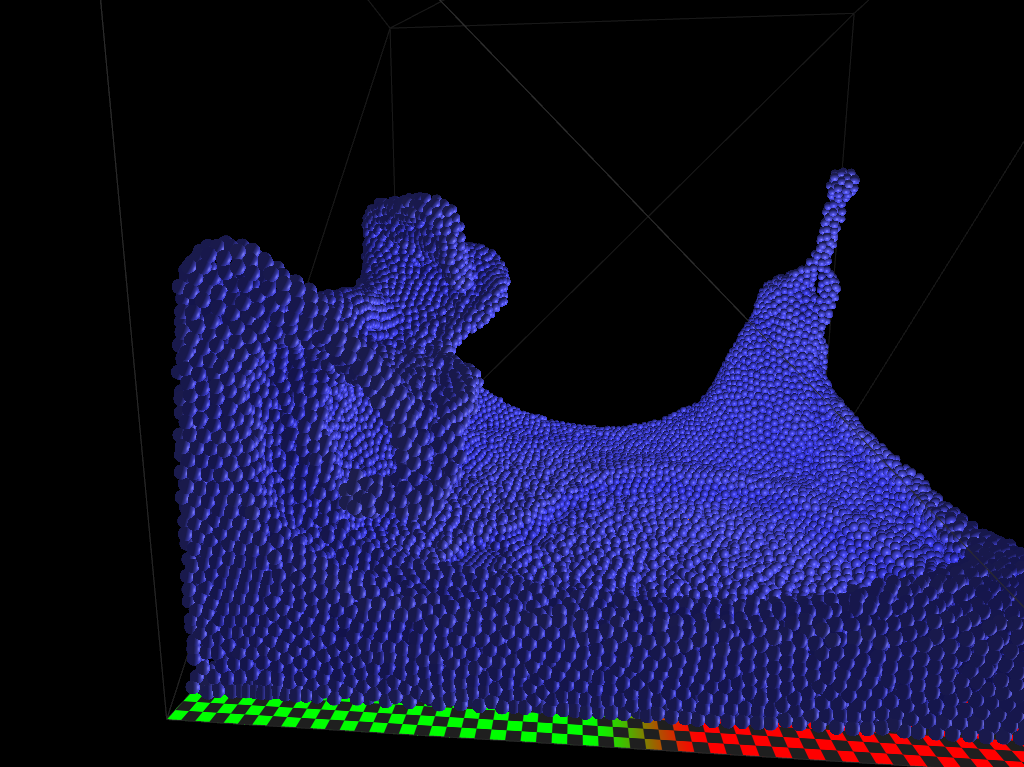
\includegraphics[width=0.9\textwidth]{img/eVorticity100.png}
  \caption{}
\end{subfigure}%
\begin{subfigure}{.5\textwidth}
  \centering
  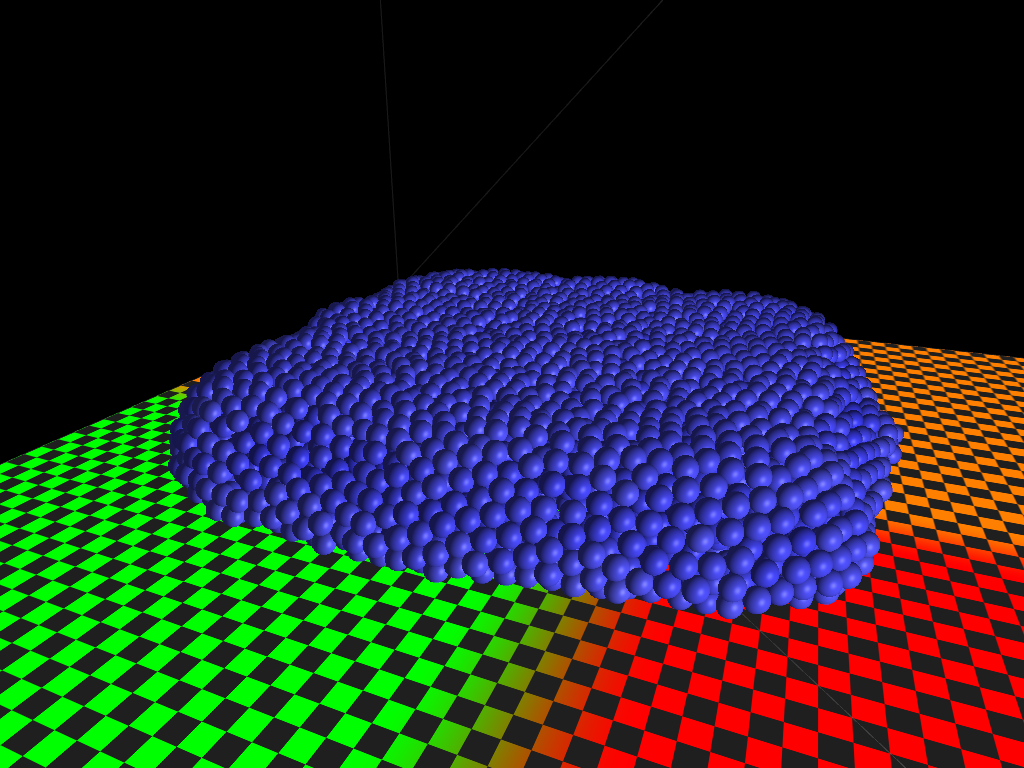
\includegraphics[width=0.9\textwidth]{img/cViscosity001.png}
  \caption{}
\end{subfigure}%
\\ \\
\centering
\begin{subfigure}{.5\textwidth}
  \centering
  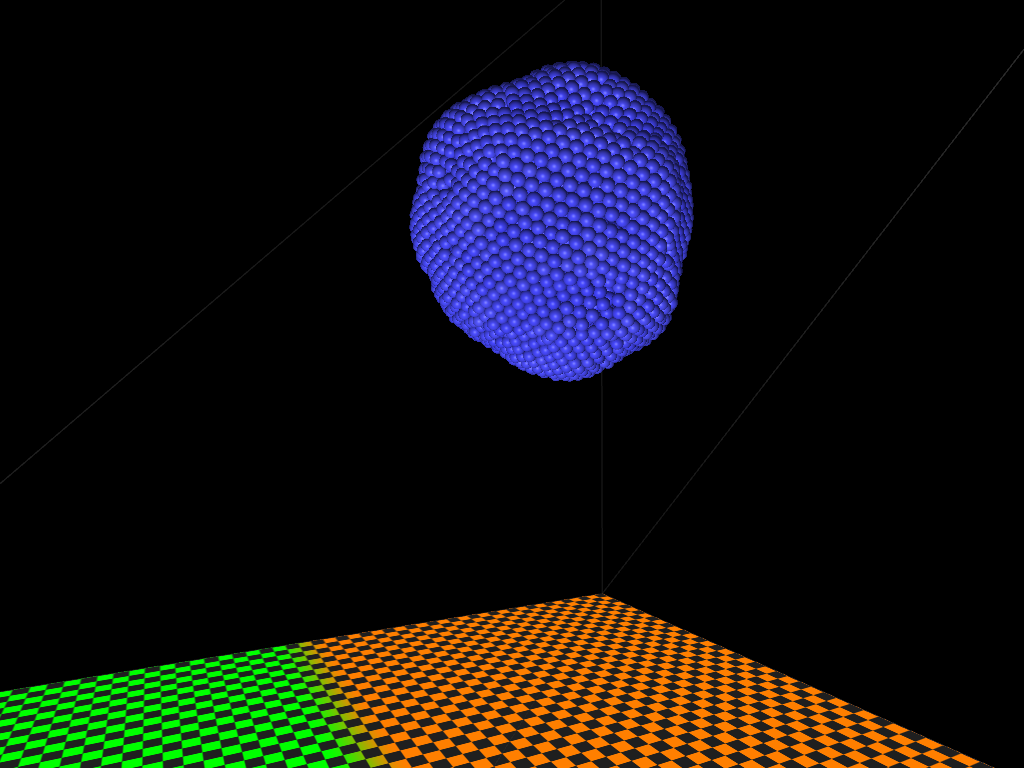
\includegraphics[width=0.9\textwidth]{img/gravity0.png}
  \caption{}
\end{subfigure}%
\begin{subfigure}{.5\textwidth}
  \centering
  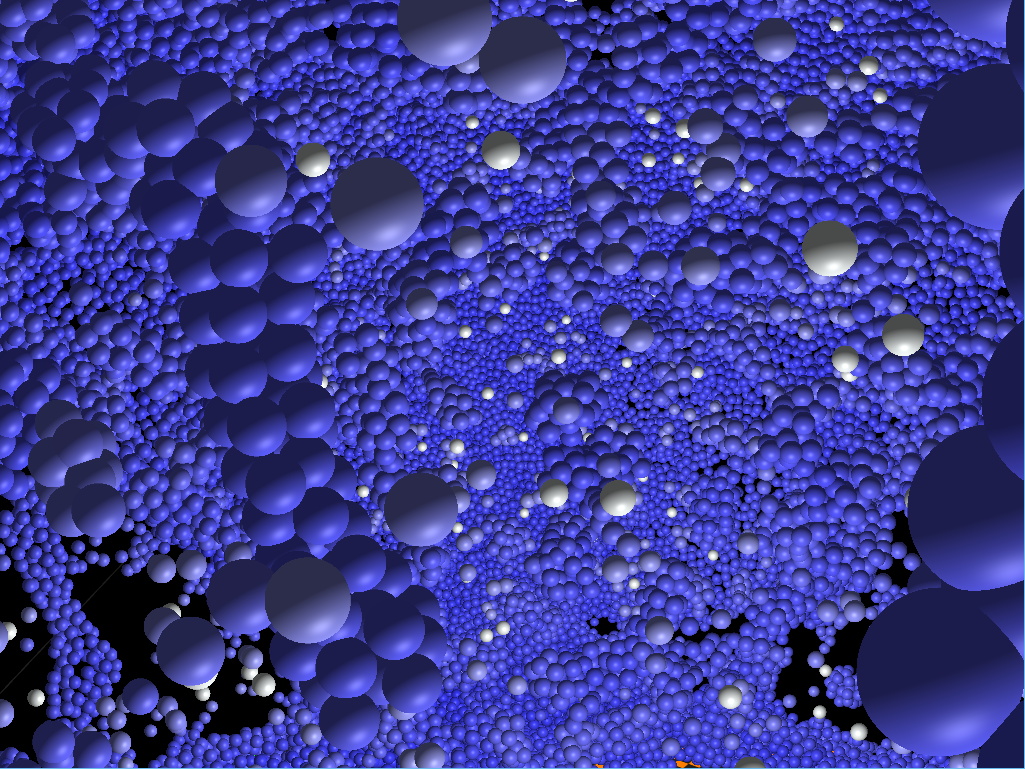
\includegraphics[width=0.9\textwidth]{img/closeupAfterExplosion.png}
  \caption{}
\end{subfigure}%

\caption{The snapshot in (a) shows the fluid when there is a bit higher vorticity, (b) when there is high viscosity, (c) when there is 0 gravity and (d) is taken after two boxes of fluid have spawned inside each other, resulting in an explosion where the particles blob together after a while.}
\label{fig:result0}
\end{figure}

\begin{figure}[H]
\centering
\begin{subfigure}{.9\textwidth}
  \centering
  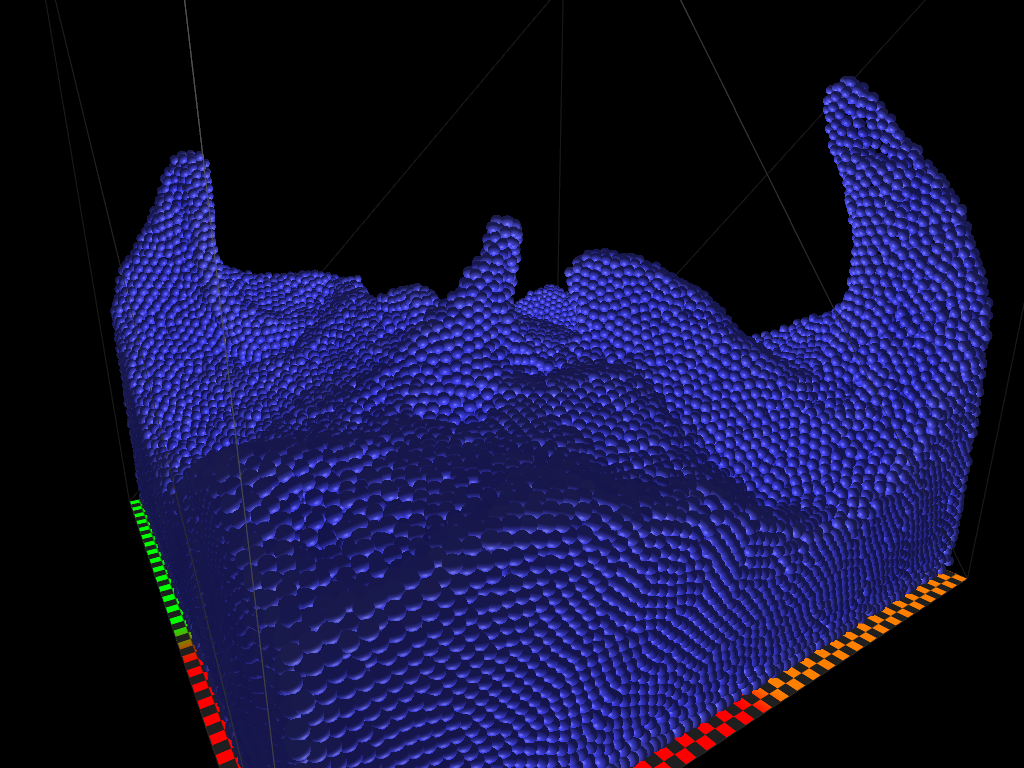
\includegraphics[width=0.9\textwidth]{img/55296_edit.png}
  \caption{}
\end{subfigure}%
\\
\begin{subfigure}{.9\textwidth}
  \centering
  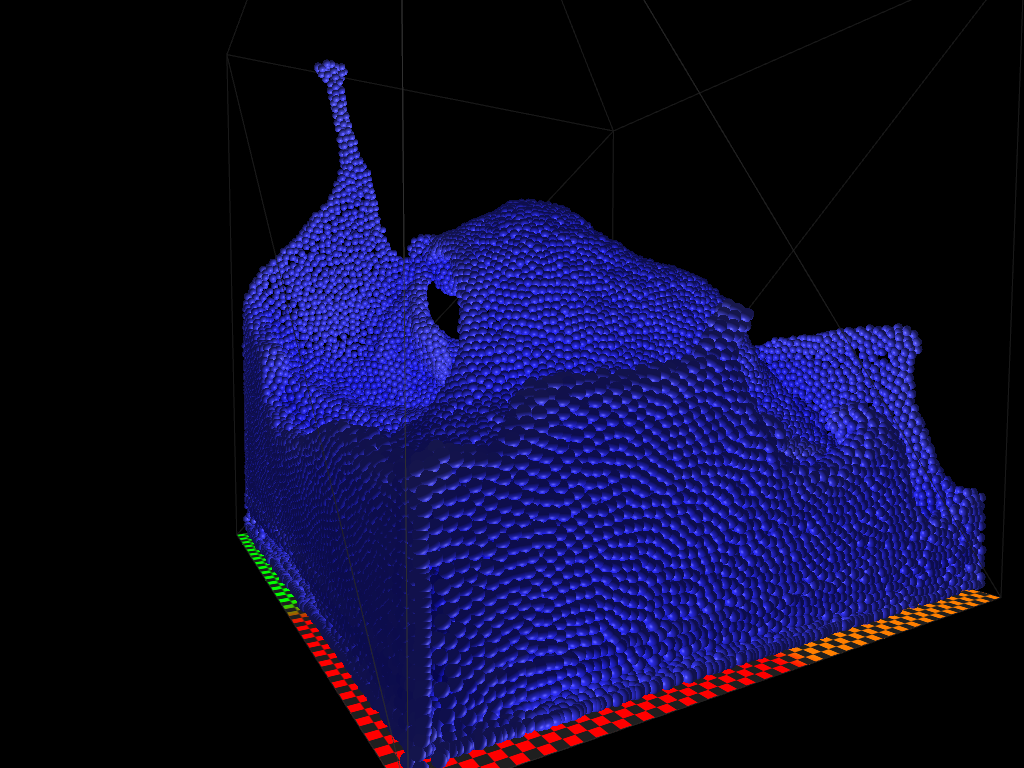
\includegraphics[width=0.9\textwidth]{img/3Nieghbours_55size.png}
  \caption{}
\end{subfigure}%

\caption{Two snapshots of our simulation, where (b) involves neighbouring particles at a larger distance resulting in slightly more curls than (a), this is due to the vorticity.}
\label{fig:result}
\end{figure}

\begin{center}
  \captionof{table}{Performance when varying the number of particles on different GPUs}
  \label{tb:fr_overview_results}
  \resizebox{\columnwidth}{!}{%
    \begin{tabular}{ | l | l | l | p{5cm} |}
      \hline
      GPU & Number of Particles & Framerate \\ \hline
      GTX - & 0 & 0 FPS \\ \hline
      GTX - & 0 & 0 FPS \\ \hline
      GTX - & 0 & 0 FPS \\
      \hline
    \end{tabular}
  }
\end{center}


\newpage 

\section{Discussion}
Our implementation of a fluid simulation using PBD was able
to achieve real-time performance for a large number of particles even while
running on laptop grade hardware. By varying parameters such as vorticity and
viscosity different fluid behaviors can be achieved ranging from thick slow
moving substances to quick and turbulent water.

In order for the simulation to be running in real time it was necessary to
exploit high levels of parallelism. Initial tests were conducted in the form
of single threaded applications running on the CPU but we were only able to
simulate less than 500 particles before the framerate became unacceptably low.
Even running the simulation in a multithreaded manner on modern CPUs capable of
8 or more concurrent tasks would not be sufficient to achieve the desired
performance. The solution to this problem was to utilize the massively parallel
architecture of current GPUs that are often times
capable of over 1000 simultaneously executing tasks. The downside to using GPUs
is that due to their unique architecture they make creating programs for them
more difficult than something running on a CPU.

It is interesting to note that the number of stabilization and solver iterations had very little impact on the final results for us as only one iteration of each were sufficient in order to run stable simulations.

\subsection{Future work}
PBD is not limited to simulating
fluids and can be used to model a large variety of behaviors. The possibilities
of PBD are only limited to the number of constraints that
can be expressed. It would be of interest to further develop our software to
handle materials such as cloth as described in~\cite{muller2007position} using
stretching constraints or deformation of objects~\cite{muller2005meshless} by
incorporating shape matching constraints.

It would also be of interest to further extend the fluid simulation as
described in~\cite{macklin2014unified} to allow for fluids of varying densities
to interact. This would include changing how density is estimated between
neighbouring particles to accommodate for a per particle variation in density
contribution. The result of this would be that phenomena such as oil floating
on top of water could be simulated.

In order to improve the visual presentation of the results we could apply a
fluid surface rendering scheme to the particles. One such method is presented
in~\cite{van2009screen} where a surface is constructed by rendering the depth
of the particles and applying a so called curvature flow filter. The filter has
the effect of blending the particles together and making the spherical shapes
less distinct resulting in the appearance of a smooth surface.


%----------------------------------------------------------------------------------------
% BIBLIOGRAPHY
%----------------------------------------------------------------------------------------

\newpage

\bibliographystyle{unsrt}

\bibliography{references}


%----------------------------------------------------------------------------------------

\end{document}
